%=========================================================================
% (c) Michal Bidlo, Bohuslav Křena, 2008
\chapter{Úvod}

\chapter{Teoretický rozbor}
\section{Síťové modely}

Zpracování dat síťového provozu je rozděleno do několika úrovní. Tyto úrovně jsou popsány síťovými modely.
Základním modelem je ISO/OSI, který slouží pro abstraktní rozdělení operací zpracování a jeho použití je
pouze pro akademické účely. V reálných počítačových sítích pak dominuje model TCP/IP, který má oproti
ISO/OSI modelu menší počet vrstev.

\subsection{ISO/OSI}
ISO/OSI model je rozdělen na sedm vrstem.

\begin{enumerate}
	\item{Fyzická vrstva / Vrstva síťového rozhraní}
	\item{Linková vrstva}
	\item{Síťová vrstva}
	\item{Transportní vrstva}
	\item{Relační vrstva}
	\item{Prezentační vrstva}
	\item{Aplikační vrstva}
\end{enumerate}

\begin{figure}[!htb]
\centering
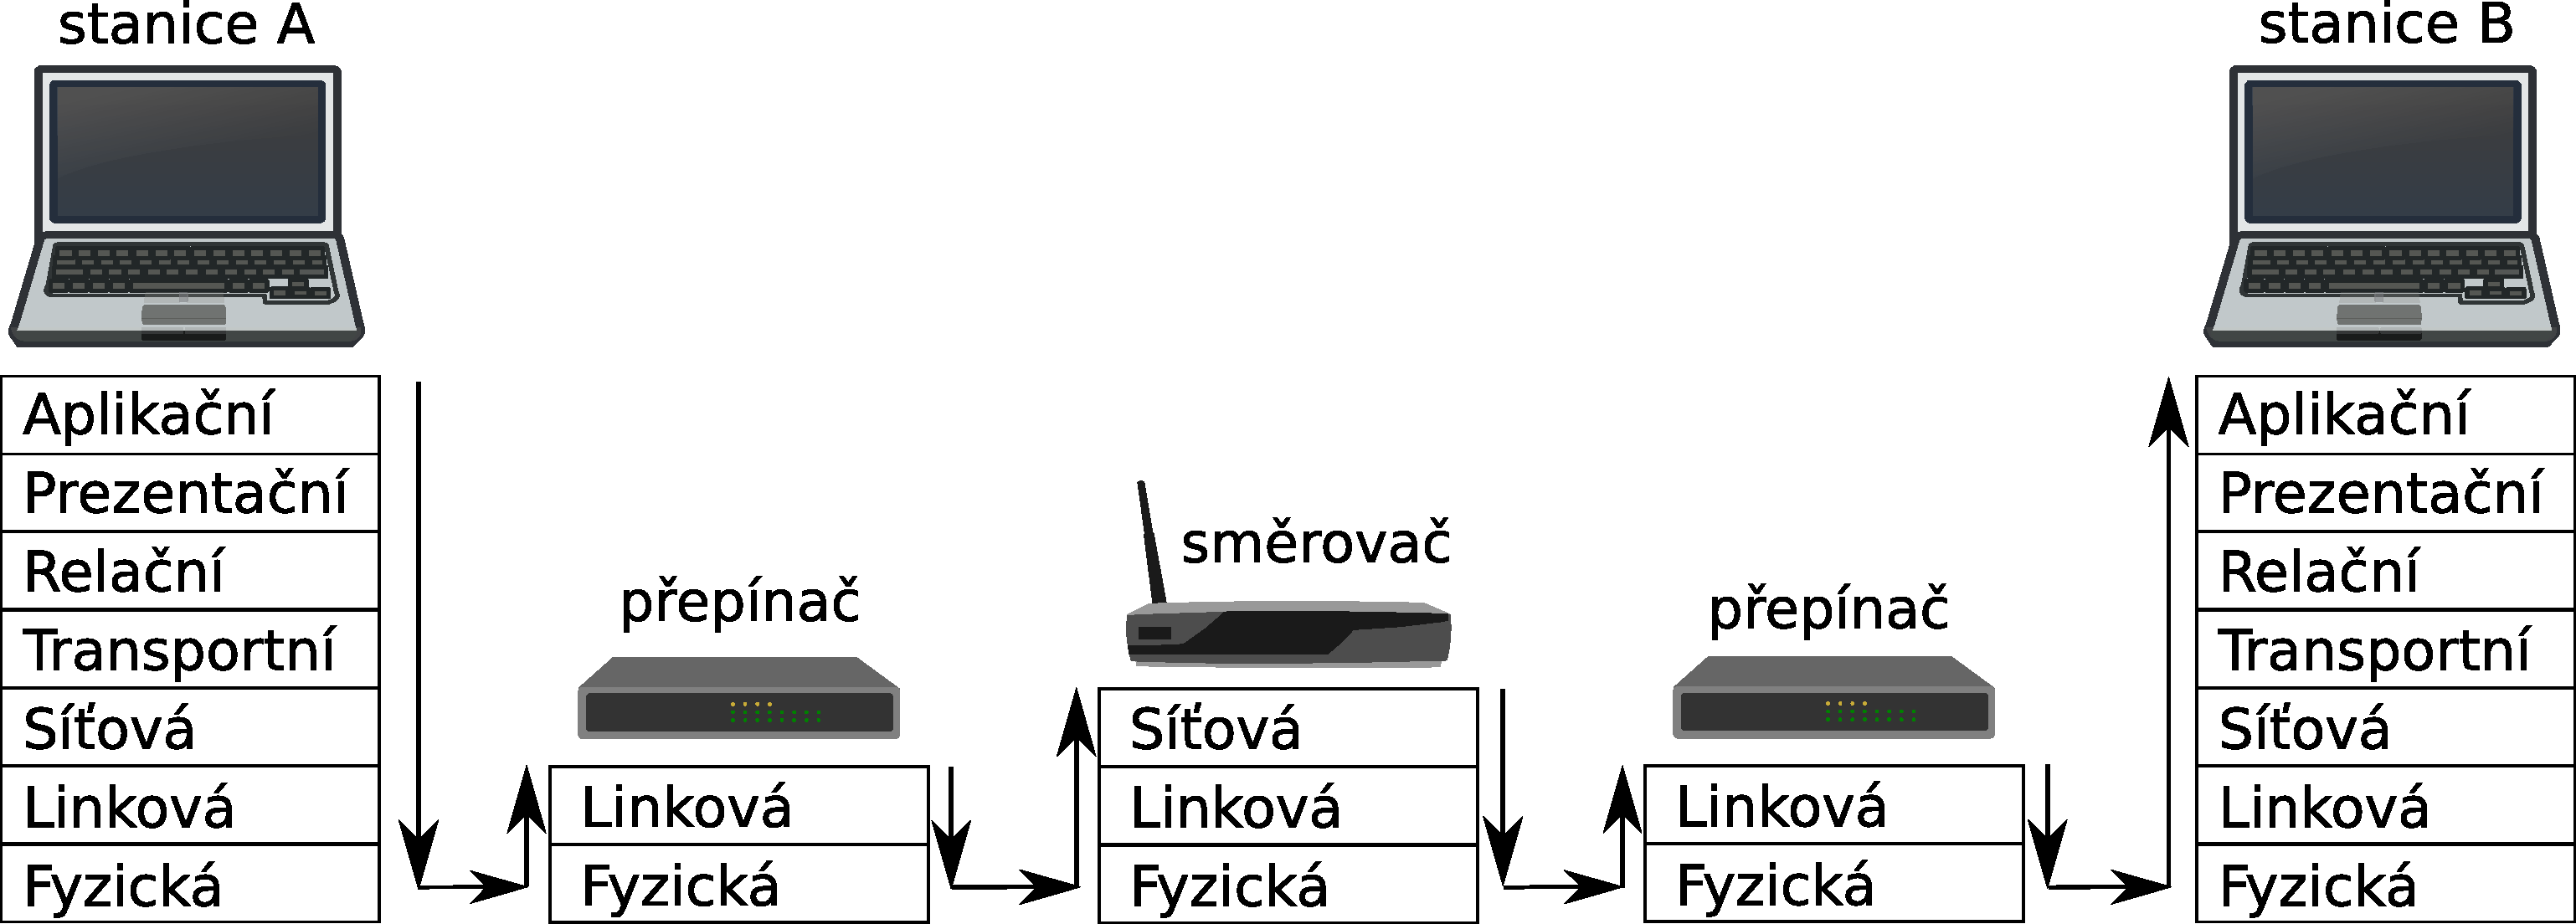
\includegraphics[scale=.25]{fig/layers.pdf}
\caption{Znázornění průchodu dat počítačovou sítí v modelu ISO/OSI}
\label{fig:layers}
\end{figure}

\subsection{TCP/IP}
TCP/IP model se skládá pouze ze čtyř vrstev.

\begin{enumerate}
	\item{Vrstva síťové rozhraní}
	\item{Síťová vrstva}
	\item{Transportní vrstva}
	\item{Aplikační vrstva}
\end{enumerate}

\subsection{Popis vrstev síťových modelů}

\subsubsection{Fyzická vrstva / Vrstva síťového rozhraní}\label{layers:physical}
Nejnižší vrstva v obou zmíněných modelech pracuje s daty na úrovni bitů a stará se o
jejich přenos po přenosovém médiu. Protokoly této vrstvy definují signály, které reprezentují data
a tudíž jde o protokoly implementované již v hardware síťových zařízení.

\subsubsection{Linková vrstva}\label{layers:link}
Linková vrstva je druhá nejnižší vrstva síťových modelů. Tato vrstva se stará o datovou komunikaci
obecně mezi několika uzly, které jsou přimo spojeny. Spojení může být jak fyzickým vodiček tak i
bezdrátovou technologií. Nejrozšířenější technologií pro fyzické spoje je Ethernet, pro bezdrátové spoje
je to standard IEEE 802. Datová jednotka na linkové vrstvě se nazývá rámec a nese v sobě kromě
zapouzdřených dat vyšších vrstev také informace o kontrolním součtu dat a adresování pomocí MAC adres.
MAC adresa je adresa fyzického zařízení, které pracuje na této vrstvě.
Adresování MAC adresou slouží pro identifikaci zařízení, které se nacházejí ve stejné počítačové síti
a za hranici této sítě se již používá IP adresace, které je vysvětleno v necházející kapitole \ref{layers:network}
Nekoncová síťová zařizení která pracují na této vrstvě se nazývaji huby.

\subsubsection{Síťová vrstva}\label{layers:network}
Na této vrstvě probíhá komunikace za využití IP adres. Prvky používané na této vrstvě jsou nazývaný routery.
Účelem těcho zařízení je směrování paketů procházejících sítí. K tomu využívají směrovací tabulku na optimalizace jejího prohledávání
se věnuje část této práce zabývající se problémem vyhledávání nejdelšího shodného prefixu.
Datové struktury jsou pojmenované pakety.
Pakety obsahují

\subsubsection{Transportní vrstva}
Transportní vrstva pracuje s datovou strukturou zvanou segmenty. Obsahují informace jako je kontrolní součet pro zjištění integrity dat,
pořadové číslo rámce pro spojení dat, která byla na cestě k cíli rozdělena na více částí a také obsahuje čísla portů
pro určení uživatelských aplikací, která data odeslala a která je na druhém konci má přijmout.

Transportní vrsta (a všechny vyšší) se tradičně již nevyskytuje na síťových zařízeních, která se starají o provoz.
Slouží až pro koncové stanice aby mohli určit program, kterému budou data předána.

\subsubsection{Relační vrstva}


\subsubsection{Prezentační vrstva}


\subsubsection{Aplikační vrstva}
Aplikační vrstva je vrstva, kde pracují uživatelské aplikace.
Na této vrstvě může docházet ke kontrole přenášeného obsahu a k detekci možný útoků na uživatelské aplikace.



\section{Časově kritické operace}
S neustálím zvyšováním požadavků na rychlost síťového připojení také rostou nároky na rychlost
algoritmů, které na síťových zařízeních pracují. Při rychlostech, které jsou dnes reálné je problém se zpracováním
síťových operací, které mají k dispozici pouze několik desítek procesorových instrukcí pro zpracování jednoho požadavku
pokud bereme v úvahu veřejností používané procesory.

Proto v posledních letech nabírá na obrátkách trend pro využítí ASIC čipů nebo programovatelných hradlových polí.
Tyto prvky totiž umožňují rychlejší zpracování s řádově menšími požadavky.
Tohoto rychlostního rozdílu je dosaženo právě díky specializaci čípů na provádění jedné specializované operace na což jsou uzpůsobeny
narozdíl od obecných procesorů, které musejí zvládat mnohem větší repertoár operací.

\subsection{Teorie}

Pro operace hledání hledání podřetězců a zpracování regulárních výrazů popsaných v kapitolách N a N
jsou použity konečné automaty.

Konečný automat je uspořádaná pětice

\begin{huge}
\begin{equation}\cite{meduna}
A=(Q,\Sigma, \sigma,q_0 ,F)
\end{equation}
\end{huge}

Pro nedetermnistický konečný automat platí, že
\begin{itemize}
\item{\tt{Q} je množina stavů}
\item{\tt{$\Sigma$} je množina vstupních symbolů}
\item{\tt{$\sigma$} je přechodová fce $Q \times \{\Sigma \cup \epsilon\} \rightarrow Q$}
\item{\tt{$q_0 \subseteq Q$} je množina počátečních stavů}
\item{\tt{$F \subseteq Q$} je množina konečných stavů}
\end{itemize}

Pro nedetermnistický konečný automat platí, že

\begin{itemize}
\item{\tt{Q} je množina stavů}
\item{\tt{$\Sigma$} je množina vstupních symbolů}
\item{\tt{$\sigma$} je přechodová fce $Q \times \Sigma \rightarrow Q$}
\item{\tt{$q_0 \in Q$} je počáteční stav}
\item{\tt{$F \subseteq Q$} je množina konečných stavů}
\end{itemize}
% todo zdroj https://books.google.cz/books?id=s7gEErax71cC&vq=determinization&hl=cs&source=gbs_navlinks_s
Determinizace automatu se provádí pomocí dvou funkcí.
První z nich je epsilon uzávěr a druhá je tzv move funkce.

\subsubsection{epsilon-uzávěr} %todo nezobrazuje se jako nadpis
asda

\begin{algorithm}[H]
	\KwData{Počáteční stav nedeterministeckého automatu}
	\KwResult{Deterministický konečný automat}
	state $\leftarrow$ EpsilonClosure(nfa-start)\;
	unprocessed.push(state)\;
	\While{!unprocessed.empty()}
	{
		state $\leftarrow$ unprocessed.pop()\;
		\ForEach{symbol $s$ in $input\_alphabet$}
		{
			x $\leftarrow$  move(processing state, s)\;
			y $\leftarrow$  EpsilonClosure(x)\;
			% todo dopsat
		}
	}
	\caption{Determinize konečného automatu}
\end{algorithm}

\subsubsection{determinizace} %todo nezobrazuje se jako nadpis

\subsection{Regulární výrazy}

Regulární výrazy slouží pro popis operací nad jazykem.
Jazyk je je definovaný jako blah nad vstupní abecedou.
Jazek je definovaný jako iterace nad vstupní abecedou.
Iterace může  být neutrální nebo kladná.
V neutrální iteraci jazyka je oproti pozitivní iteraci zahrnut i symbol $\epsilon$,
který reprezentuje prázdný znak/řetězec.
Iterace jazyka se označuje jako $L^n$ kde \texttt{n} je označení iterace jazyka.
iterace $L^0$ obsahuje pouze jeden symbol a tím je $\epsilon$
$\epsilon$ také reprezentuje prázdný řetězec. Prázdný řetězec se může skládat z nekonečné posloupnosti $\epsilon$
Vstupní abeceda je množina symbolů.

Regulární výrazy jsou poté operace nad regulárními jazyky.
Regulární výrazy mají stejnou  vyjadřovací schopnost jako konečné automaty a pro digitální zpracování
regulárních výrazů se vždy používají konečné automaty.

Operace regulárních výrazů jsou následující

\begin{itemize}
\item{$\emptyset$ je regulární výraz reprezentující prázdnou množinu}
\item{$\epsilon$ je regulární výraz reprezentující $\{\epsilon\}$}
\item{$a, a \in \Sigma$ je regulární výraz reprezentující $\{a\}$}
\item{$(r \cdot s)$ je regulární výraz reprezentující $RS$}
\item{$(r | s)$ je regulární výraz reprezentující $R \cup S$}
\item{$(r*)$ je regulární výraz reprezentující R*}
 % todo zdroj https://books.google.cz/books?id=s7gEErax71cC&vq=determinization&hl=cs&source=gbs_navlinks_s
\end{itemize}

Znak operace konkatenace % TODO přidat referenci na item nahoře
se čast vynechává a je uvažován implicitně.

Regulární výrazy implementované v této knihovně rozšiřují množinu operací o syntaktická pozlátka

\begin{itemize}
	\item{$[abc]$ je výčet znaků, které se na vstupu mohou vyskytnout a automat je v aktuální stavu dokáže zpracovat. Je to zkrácený tvar zápisu $(a|b|c)$}
	\item{$a+$ je definováno jako pozitiní iterace, tedy $1..N$ opakování}
	\item{$a?$ je definováno jako $0..1$ iterací}
\end{itemize}

\begin{algorithm}
	\KwData{start-state, text}
	\KwResult{keyword}
	state = start-state\;
	\For{position $\leftarrow$ 0 \KwTo text.length}
	{
		\lWhile{goto(state, text[position]) == FAIL}{state $\leftarrow$ state.failure}
		\lIf{state.isMatch}{\Return state.keyword}
	}
	\Return NOT-MATCH\;
	\caption{Algoritmus procházení textu a hledání podřetězců}
\end{algorithm}

\cite{aho}

\begin{algorithm}
	\KwData{bspl-root, hash-table, ip, ip-length}
	\KwResult{routing rule}
	prefix-length $\leftarrow$ ip-length\;
	prefix-change $\leftarrow$ ip-length\;
	\Repeat{prefix-change > 0}
	{
		bits $\leftarrow$ get-prefix-bits(ip, prefix-length)\;
		item $\leftarrow$ hast-table.get(bits)\;
		prefix-change $\leftarrow$ prefix-change \texttt{>>} 1\;

		\If{item == NULL}{prefix-length $\leftarrow$ prefix-length - prefix-change\;}
		\ElseIf{item.type == PREFIX}{prefix-length $\leftarrow$ prefix-length + prefix-change\;}
		\lElse{break}
	}
	\lIf{item == NULL}{\Return bspl-root.default-rule}
	\caption{Hledání nejdelšího shodného prefixu algoritmem Binary search on prefix length}
\end{algorithm}

\cite{bspl}

\begin{algorithm}
	\KwData{tbm-root, ip, ip-length}
	\KwResult{routing rule}
	node $\leftarrow$ tbm-root\;
	position $\leftarrow$ 0\;
	\Repeat{BIT(parent.external, bits)}
	{
		bits $\leftarrow$ get-stride-bits(ip, position, prefix-length)\;
		position $\leftarrow$ position + STRIDE\;

		\If{isRule(node.internal, bits)}
		{
			longest-match = node\;
		}

		index $\leftarrow$ ones(node.external, bits)\;
		parent $\leftarrow$ node\;
		node $\leftarrow$ node.external[index]\;
	}
	\Return longest-match\;
	\caption{Hledání nejdelšího shodného prefixu algoritmem TreeBitmap}
\end{algorithm}

\cite{tbm}

\subsection{Hledání nejdelšího prefixu}
Hledání nejdelšího shodného prefixu se používá při směrování paketů.
Pro docílení nejlepší efektivity při přeposílání paketů je nutné znát co nejpřesněji další místo, na které je paket třeba doručit.
Toho je řešeno prohledáváním routovací tabulky.
Pro dosažení větší rychlosti je routovací tabulka v paměti směrovače uložena v jiných strukturách, které tabulce neodpovídají.
V této práci jsou pro uložení routovací tabulky využity algoritmy {\tt Binary search on prefix length} a {\tt TreeBitmap}.
Oba jsou variací obecně n-árního stromu.

Při chybě alokace dojde na rozdíl od odstatních podúloh k zanechání již vytvořené fungující struktury
a to z důvodu předpokladu, že routovací tabulka se mění v čase běhu programu

\subsection{Hledání podřetězců}
Pro hledání potřetězců je implementován algoritmus autorů Aho a Corasicové. Tento algoritmus používá pro zjištění shody s podřetězcem konceptu konečného automatu. Při každé iteraci algoritmu se provede přechod o jeden znak.

\subsubsection{Aho-Corasick}
efektivita aho-coracick algoritmu je velkým dílem závislá na tom, zda se veškerá paměť použitá k uložení vyhledávaných slov veljde do cache paměti stroje, na kterém poběží.

Na klasickém desktopovém počítači je několik vrstev cache pamětí.
Pokud budeme brát v úvahu jednotlivé vrstvy samostatně, tak do
velikost jednoho stavu automatu se může výrazně lišit v závislosti počtu následovníků a počtu
pravidel, které nejsou přímo v tomto stavu, ale jsou to podřetězce tohoto stavu.
Tyto podřetězce byly zjištěny iterativním procházením automatu od hloubky 0 a procházení tzv. failure cest, kdy každý stav navštívený failure průchodem obsahující pravidlo znamená že stav, pro který se hledá failure cesta obsahuje podpravidlo vyhovující právě tomuto stavu.
L1 se vejde XXXXX stavů automatu, což může reprezentovat právě XXX slov o délce NNNN znaků.
L2 se vejde XXXXX stavů automatu, což může reprezentovat právě XXX slov o délce NNNN znaků.
L3 se vejde XXXXX stavů automatu, což může reprezentovat právě XXX slov o délce NNNN znaků.
L4 se vejde XXXXX stavů automatu, což může reprezentovat právě XXX slov o délce NNNN znaků.

Při chybě alokace se smaže celý výraz, neexistuje předpoklad na dynamické přidávání pravidel za běhu programu

\subsubsection{Regulární výrazy}

\begin{figure}[!htb]
\centering
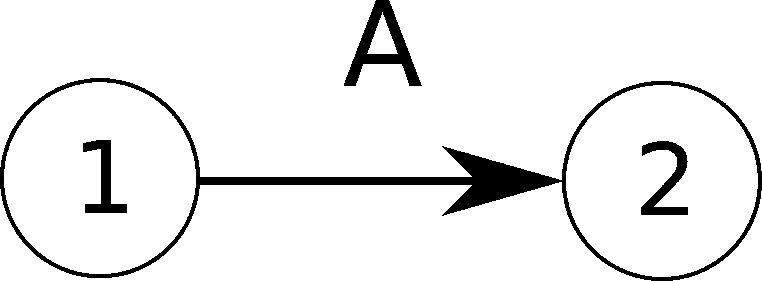
\includegraphics[scale=.25]{fig/regex-block.pdf}
\caption{Znázornění průchodu dat počítačovou sítí}
\label{fig:regex-block}
\end{figure}

\begin{figure}[!htb]
\centering
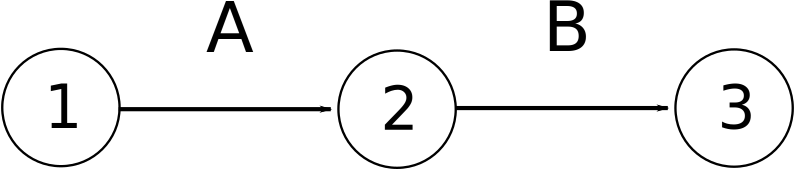
\includegraphics[scale=.25]{fig/regex-concat.pdf}
\caption{Znázornění průchodu dat počítačovou sítí}
\label{fig:regex-concat}
\end{figure}

\begin{figure}[!htb]
\centering
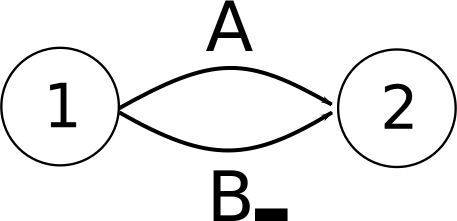
\includegraphics[scale=.25]{fig/regex-dot.pdf}
\caption{Znázornění průchodu dat počítačovou sítí}
\label{fig:regex-dot}
\end{figure}

\begin{figure}[!htb]
\centering
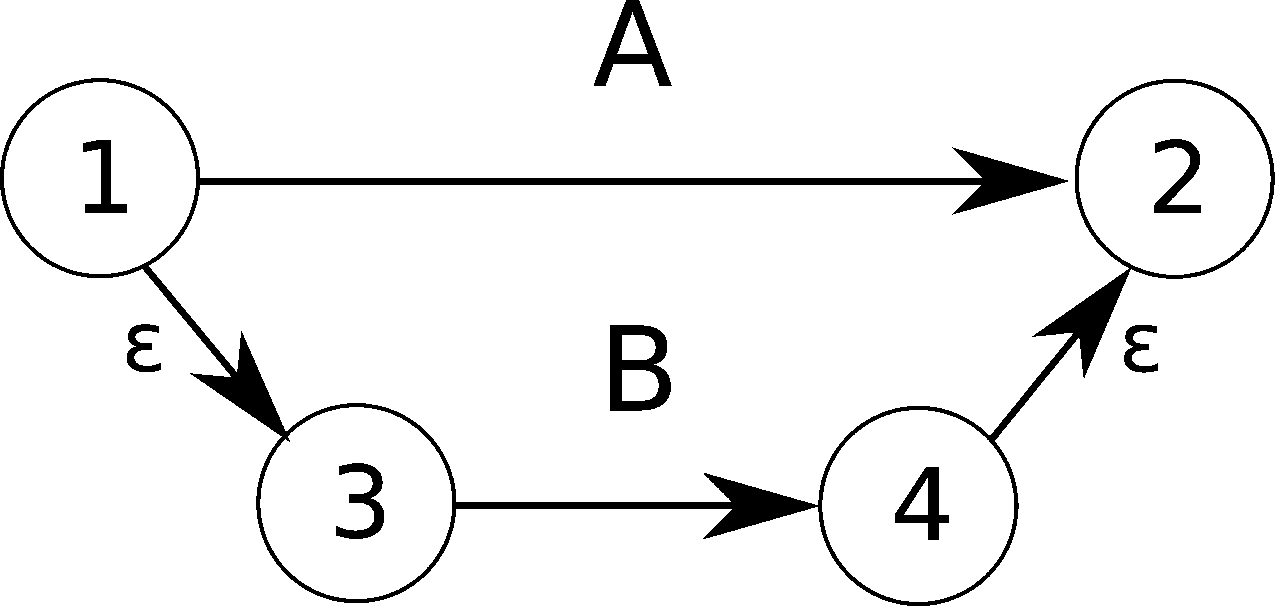
\includegraphics[scale=.25]{fig/regex-or.pdf}
\caption{Znázornění průchodu dat počítačovou sítí}
\label{fig:regex-or}
\end{figure}

\begin{figure}[!htb]
\centering
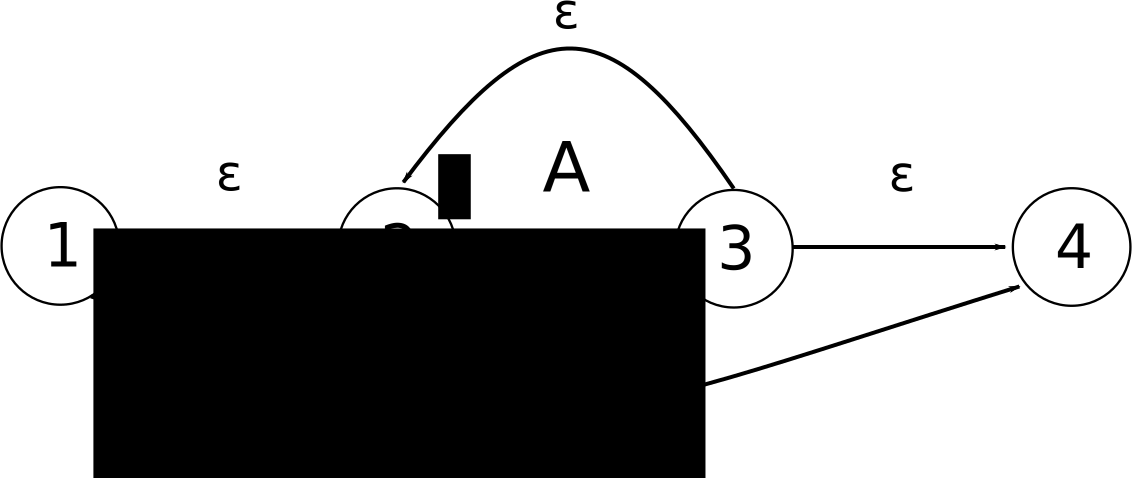
\includegraphics[scale=.25]{fig/regex-star.pdf}
\caption{Znázornění průchodu dat počítačovou sítí}
\label{fig:regex-star}
\end{figure}

\begin{figure}[!htb]
\centering
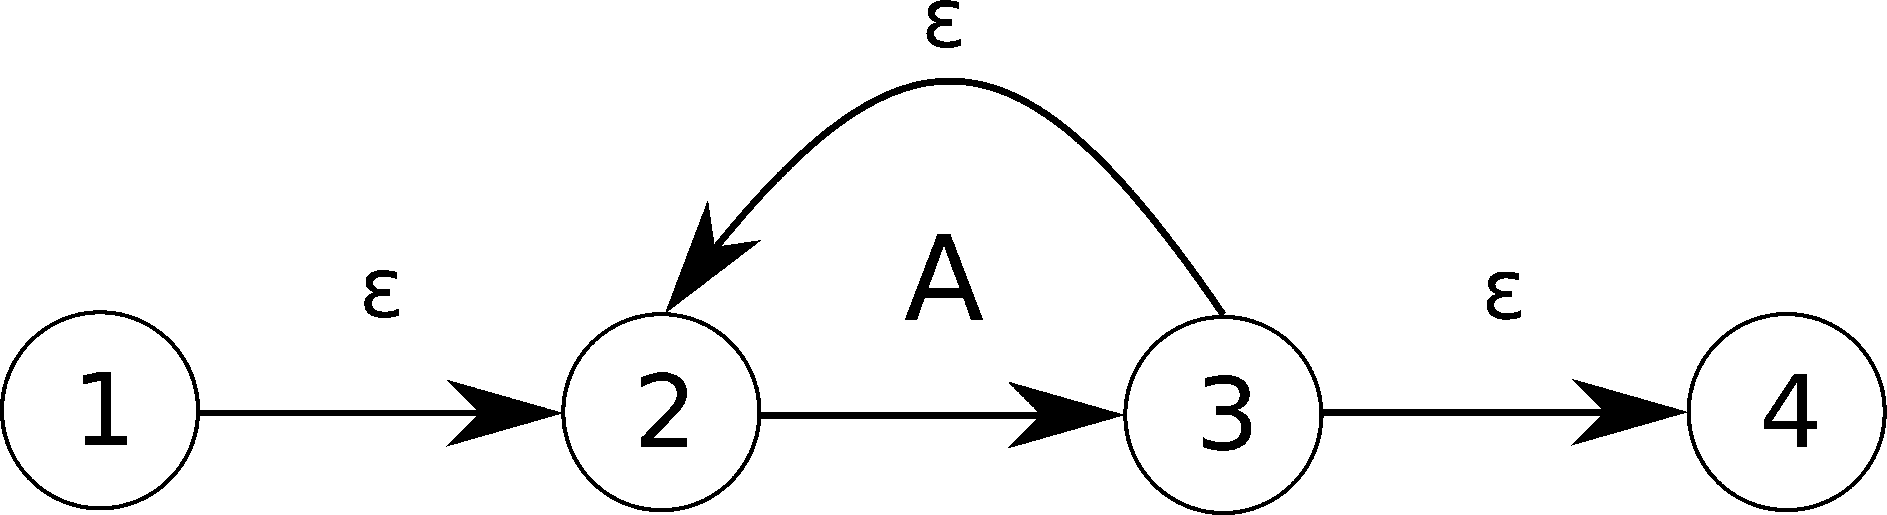
\includegraphics[scale=.25]{fig/regex-plus.pdf}
\caption{Znázornění průchodu dat počítačovou sítí}
\label{fig:regex-plus}
\end{figure}

\begin{figure}[!htb]
\centering
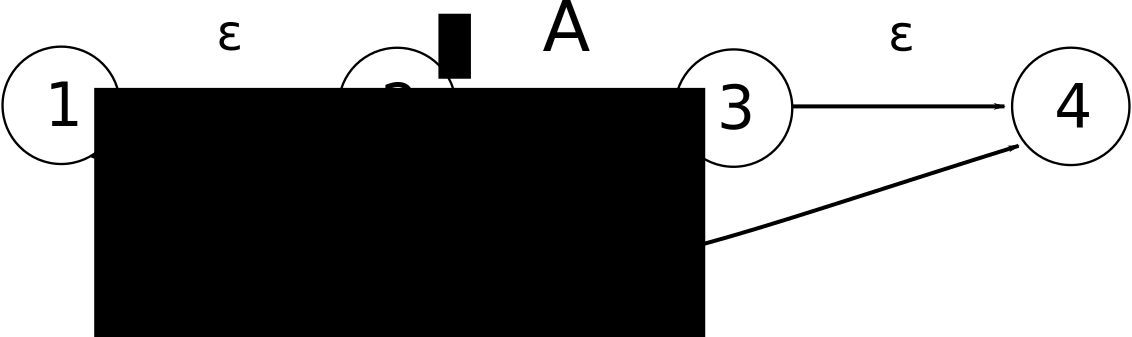
\includegraphics[scale=.25]{fig/regex-questionmark.pdf}
\caption{Znázornění průchodu dat počítačovou sítí}
\label{fig:regex-questionmark}
\end{figure}
% TODO konstrukce NFA
% TODO konstrukce DFA z NFA
% TODO konstrukce MDFA z DFA
== 3 strany

Při chybě alokace se smaže celý výraz, neexistuje předpoklad na dynamické přidávání pravidel
regulárních výrazů za běhu programu

\chapter{Návrh API knihovny}
Knihovna je navržena s důrazem na snadnou rozšiřitelnost případnými dalšími algoritmy.
Knihovna je taktéž navržena tak, aby bylo velmi snadné používat pouze jednu z operací, které knihovna implementuje.
To je vhodné pro použití v úzce specializovaných zařízení, jimž tak bude stačit menší množství paměti pro uložení knihovny.
Každá podknihovna lze vytvořit jedním příkazem ve své složce a také poskytuje vlastní rozhraní, které lze vložit do používaných algoritmů.

\begin{figure}[!htb]
\centering
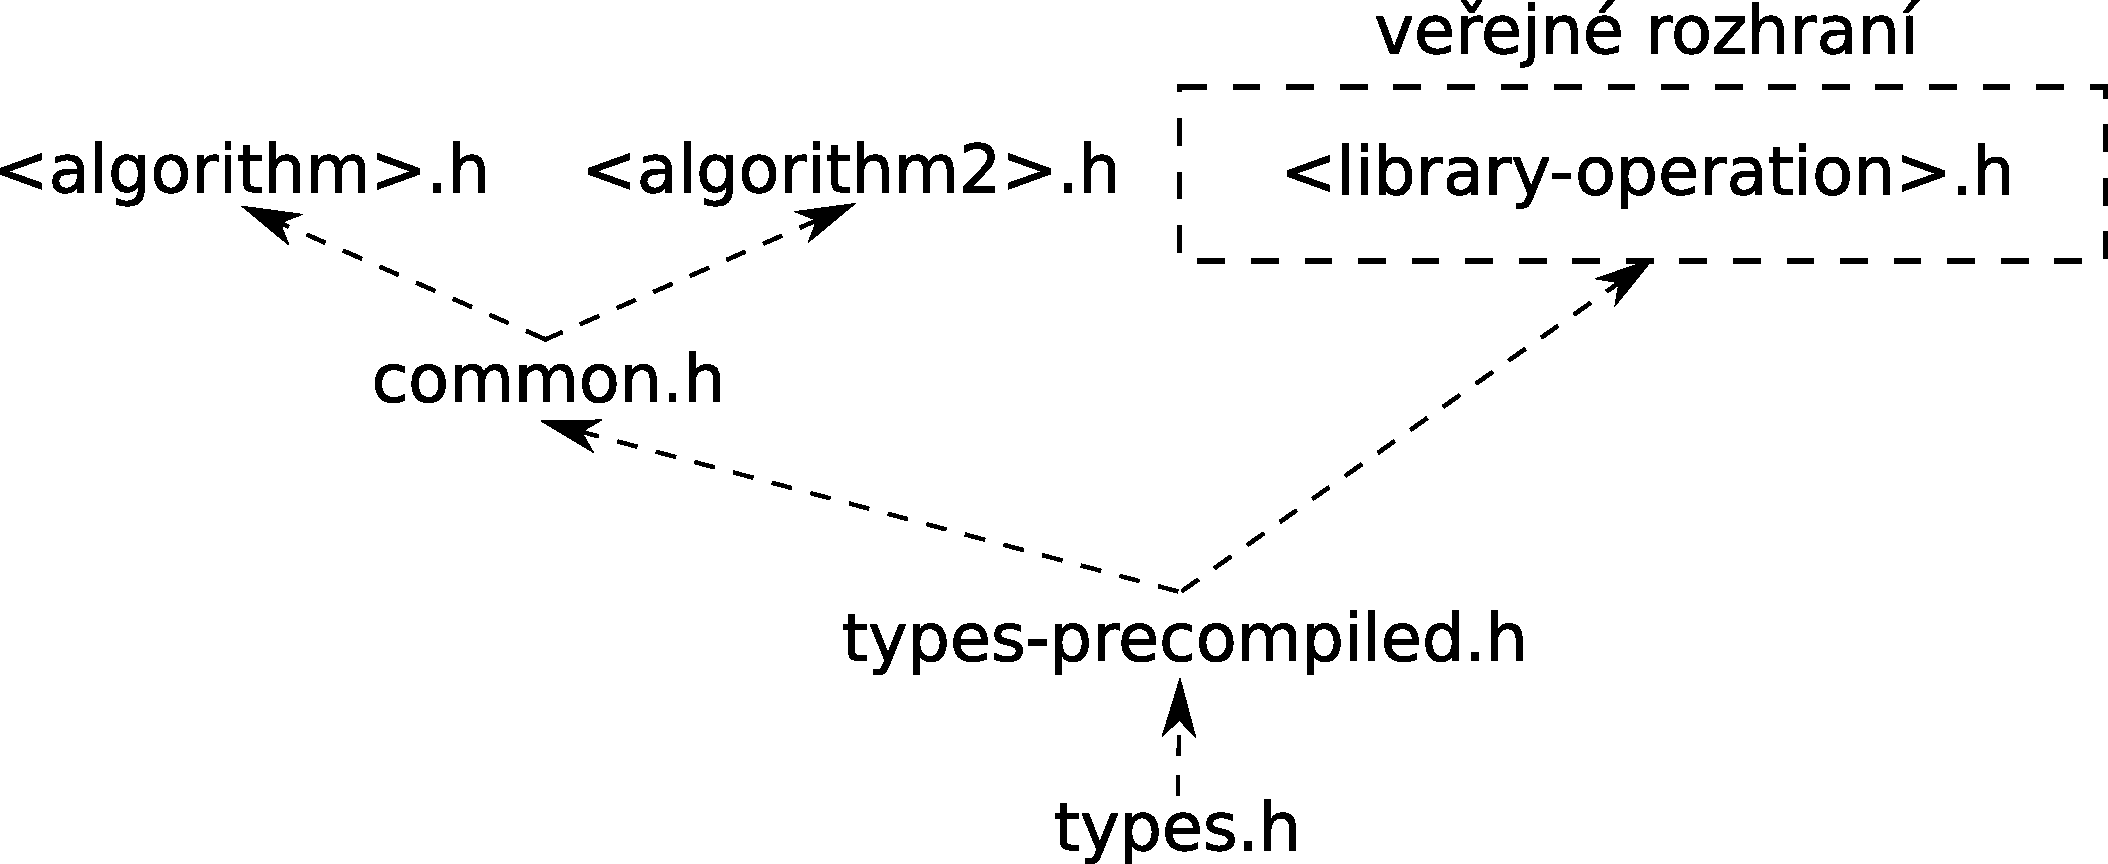
\includegraphics[scale=.25]{fig/header-dependencies.pdf}
\caption{Diagram závislostí hlavičkových souborů}
\label{fig:header-dependecies}
\end{figure}

hlavičkové soubory jsou rozděleny na veřejné a privátní rozhraní, kde privátní rozhraní je používáno pouze uvnitř knihovny. Hierarchickou strukturu je možné vidět na obrázku \ref{fig:header-dependecies}.

Jako výchozí hlavičkový soubor je použit types.h, který obsahuje definice datových struktur pro všechny algoritmy v podknihovně, které musí být viditelné i z veřejného rozhraní. Dalším souborem je types-precompiled.h, který je generován z types.h při překladu když se vybírá používaný algoritmus. common.h je hlavičkový soubor společný pro všechny algoritmy v podknihovně a algortihm.h pak obsahuje deklarace právě pro jeden konkrétní algoritmus.
sublib.h je pak hlavičkový soubor, který tvoří veřejné rozhraní ke knihovním funkcím.



Důvod pro vlastní implementaci regulární výrazů je možnost zvolit nejvhodnější algoritmus pro danou operaci.
Dalším důvodem je převod implementace do akcelerovaného hardware.
Nějvýznamějším důvod pro vlastní implementaci je provádění několika regulárních výrazů najednou na jednom vstupní textu a vracení čísla regulárního výrazu, který vstupnímu textu vyhovuje, což není možné docílit při použití stadardní implementace ze stdlib, {\tt regex}

\chapter{Výsledky}
\section{Hledání nejdelšího shodného prefixu}
U algoritmu bspl je doba vyhledání prefixu velice závislá na velikosti hešovací tabulky a proto je vhodné odhadnout počet záznamů tabulky alespoň řádově a dle toho pak nastavit velikost konstantu \tt{\_HTABLE\_SIZE} v souboru bspl.h na hodnotu, která alespoň řádově odpovídá předpodkládané velikosti hešovací tabulky.

% TODO udělat experiment na 100k záznamech a různých velikostech tabulky

\chapter{Závěr}
Závěrečná kapitola obsahuje zhodnocení dosažených výsledků se zvlášť vyznačeným vlastním přínosem studenta. Povinně se zde objeví i zhodnocení z pohledu dalšího vývoje projektu, student uvede náměty vycházející ze zkušeností s řešeným projektem a uvede rovněž návaznosti na právě dokončené projekty.

\section{Další vývoj projektu}

Jako další kroky pro vylepšení knihovny bych zvolil optimalizaci implementovaných algoritmů dle

Stress testing
- ověřit že se knihovna chová dle specifikace i při nedostaku paměti a v případech, kdy dojde k malloc nullu
a provolávají se různé funkce

%=========================================================================
